\documentclass[paper=a4, fontsize=11pt]{scrreprt}

\usepackage[T1]{fontenc}
\usepackage[german]{babel}
\usepackage{amsfonts,amsthm, amsmath}
\usepackage{siunitx}
\usepackage[]{graphicx}
\usepackage{url}
\usepackage{floatrow}
\usepackage{sectsty}
\usepackage{fancyhdr}
\usepackage[utf8]{inputenc}

\allsectionsfont{\raggedright \normalfont\scshape}
\pagestyle{fancyplain}
\fancyhead{}
\fancyfoot[L]{}
\fancyfoot[C]{}
\fancyfoot[R]{\thepage}
\renewcommand{\headrulewidth}{0pt}
\renewcommand{\footrulewidth}{0pt}
\setlength{\headheight}{13.6pt}

\numberwithin{equation}{section}
\numberwithin{figure}{section} 
\numberwithin{table}{section}

\setlength\parindent{0pt}

\newcommand{\horrule}[1]{\rule{\linewidth}{#1}}

\title{	
	\normalfont \normalsize 
	\textsc{HAW, Praktikum Rechnernetze} \\ [25pt] 
	\horrule{0.5pt} \\[0.4cm]
	\huge Protokoll 01 \\
	\horrule{2pt} \\[0.5cm]
}

\author{Sebastian, Daniel Schruhl}

\date{\normalsize\today}
\renewcommand{\thesection}{\arabic{section}}
\sisetup{range-phrase=--}
\begin{document}

\maketitle

\section{Nachrichten Ticker}

Kleine Beschreibung was das programm macht.

\subsection{Architektur}

\begin{figure}[!htb] 
  \centering
     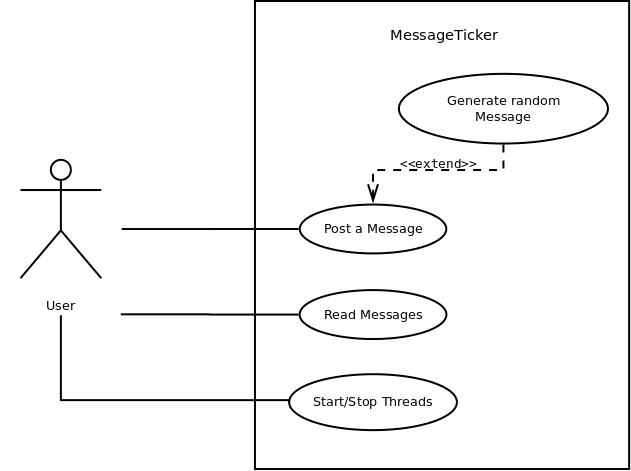
\includegraphics[width=0.5\textwidth]{resources/use-case.png}
  \caption{Anwendungsfall Diagramm MessageTicker}
  \label{fig:use-case}
\end{figure}

\begin{figure}[!htb] 
  \centering
     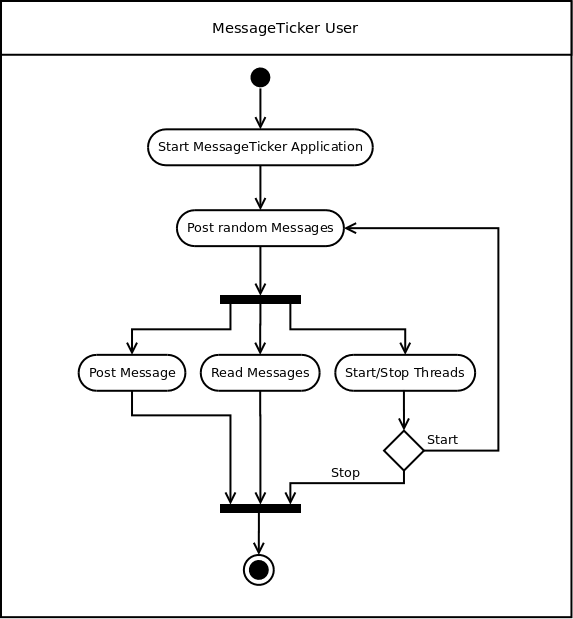
\includegraphics[width=0.5\textwidth]{resources/activity.png}
  \caption{Aktivitätsdiagramm MessageTicker}
  \label{fig:use-case}
\end{figure}

\begin{itemize}
    \item Klassendiagramm
    \item Komponenten-/Verteilungsdiagramm
    \item Sequenzdiagramm
\end{itemize} 

\section{Durchführungen im Labor}

\subsection{Webseitenabruf scimbe.de}

\begin{itemize}
	\item Dokumentieren und erklären Sie den http-Dialog.
    \item Erklären Sie exemplarisch den Aufbau (Schichten) und die Aufgabe der einzelnen Pakete.
    \item Diskutieren Sie die Frage, wie es dem Netzwerksniffer gelingt, den zugrunde liegenden TCP-Strom aus den Einzelpaketen zusammenzusetzen (Stichwort: Fragmentierung)? Können Sie die dafür nötigen Informationen identifizieren?
\end{itemize}

\subsection{Webseitenabruf https://www.google.de}

\begin{itemize}
	\item Dokumentieren und erklären Sie zunächst allgemein das veränderte Erscheinungsbild.
	\item Dokumentieren und erklären Sie die http over SSL-Kommunikation. Welche Informationen über den
Aufruf können Sie noch erkennen? Zu welchen Schichten lassen sich die Protokolle im OSI
Referenzmodell zuordnen und zu welchen im TCP/IP Modell.
	\item Erklären Sie die Rolle der Verschlüsselung aus Sicht des Netzwerkschichtenmodells.
\end{itemize}

\subsection{Webseitenabruf HTTP und HTTPS}

Stellen Sie Ihre Beobachtungen dar, erläutern diese Beobachtungen und begründen Sie Ihre Schlussfolgerungen
(Stichwort: Dienstzugang).

\subsection{IP-Adressen und Pings}

Nennen Sie im Protokoll ihre nutzbaren IP Adressen, Ihre Netzadressen und Ihre Broadcastadressen. und
beschreiben Sie Ihre Beobachtung.

\end{document}